\documentclass{standalone}
\usepackage{PhysicalChemistryNote}
\begin{document}
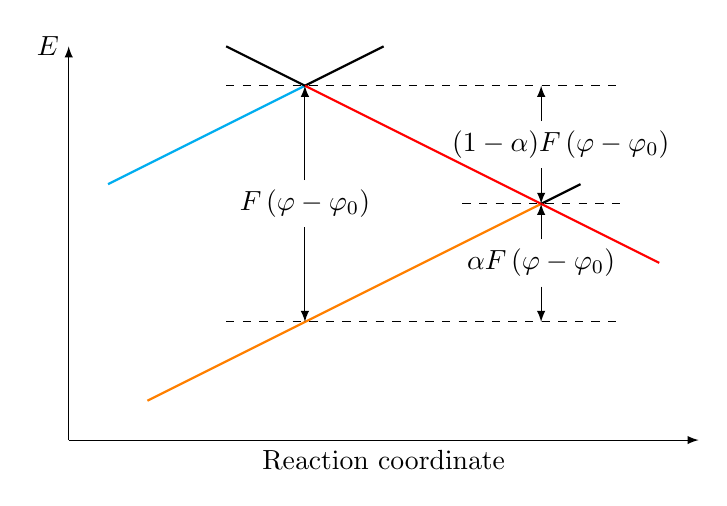
\begin{tikzpicture}
    \draw[-latex] (0,0)--(8,0);
    \node[below] at (4,0) {Reaction coordinate};
    \draw[-latex] (0,0)--(0,5) node[left] {$E$};
    \draw[thick,cyan,domain=0.5:3] plot[smooth] (\x,{0.5*\x+3});
    \draw[thick,domain=3:4] plot[smooth] (\x,{0.5*\x+3});
    \draw[thick,orange,domain=1:6] plot[smooth] (\x,{0.5*\x});
    \draw[thick,domain=6:6.5] plot[smooth] (\x,{0.5*\x});
    \draw[thick,red,domain=3:7.5] plot[smooth] (\x,{-0.5*\x+6});
    \draw[thick,domain=2:3] plot[smooth] (\x,{-0.5*\x+6});
    \draw[dashed] (2,4.5)--(7,4.5);
    \draw[dashed] (5,3)--(7,3);
    \draw[dashed] (2,1.5)--(7,1.5);
    \node at (3,3) {$F\left(\varphi-\varphi_0\right)$};
    \draw[-latex] (3,3.3)--(3,4.5);
    \draw[-latex] (3,2.7)--(3,1.5);
    \node at (6,2.25) {$\alpha F\left(\varphi-\varphi_0\right)$};
    \draw[-latex] (6,2.55)--(6,3);
    \draw[-latex] (6,1.95)--(6,1.5);
    \node at (6.25,3.75) {$(1-\alpha)F\left(\varphi-\varphi_0\right)$};
    \draw[-latex] (6,4.05)--(6,4.5);
    \draw[-latex] (6,3.45)--(6,3);
    
\end{tikzpicture}
\end{document}